\documentclass{article}

\usepackage{commath}
\usepackage{graphicx}
\usepackage{fullpage}
\usepackage{subcaption}
\usepackage{units}
\usepackage{hyperref}
\usepackage{siunitx}
\usepackage{listings}
\usepackage{multicol}
\usepackage{bm}
\usepackage{appendix}
\usepackage{textcomp}
\usepackage{gensymb}
\usepackage{booktabs}

\lstset{columns=fullflexible,basicstyle=\ttfamily}

\allowdisplaybreaks

\DeclareMathOperator*{\argmin}{argmin}

\title{
	Time stretching of the GeV emission of GRBs: Fermi LAT data vs geometrical model
}

\author{
	Maxim S. Piskunov$^{1,2}$\thanks{\href{mailto:maxit@ms2.inr.ac.ru}{maxit@ms2.inr.ac.ru}} ~and
	Grigory I. Rubtsov$^{2}$\thanks{\href{mailto:grisha@ms2.inr.ac.ru}{grisha@ms2.inr.ac.ru}} \\
	{\small $^{1}$Faculty of Physics, Moscow State University, Moscow, Russia}\\
	{\small $^{2}$Institute for Nuclear Research of the RAS, Moscow, Russia}
}

\begin{document}
\begin{flushright}  
INR-TH/2014-034
\end{flushright}
\vskip -0.9cm
{\let\newpage\relax \maketitle}

\begin{abstract}
	It is known that the high energy $(> \unit[100]{MeV})$
        emission of gamma-ray bursts is delayed with respect to the
        low energy emission.  However, the dependence of light curves
        on energy has not been studied for the high energy bands.  In
        this paper we consider the bursts observed by Fermi-LAT from
        2008 August 4 to 2011 August 1, for which at least $10$
        photons were observed with the energy greater than
        $\unit[1]{GeV}$. These include $4$ bursts: GRB 080916C, GRB
        090510, GRB 090902B, and GRB 090926A.  We use the
        Kolmogorov-Smirnov test to compare the light curves in the two
        bands, $\unit[100]{MeV} < E < \unit[1]{GeV}$ and
        $E > \unit[1]{GeV}$. For GRB 080916C and GRB
        090510 the light curves in the two bands are statistically
        compatible. However, for GRB 090926A, the higher-energy light
        curve is stretched compared to the lower-energy one with a
        statistical significance of $3.3 \sigma$ and, for GRB 090902B,
        on the contrary, the lower-energy curve is stretched with $2.3
        \sigma$ significance. We argue that the observed diversity of
        stretching factors may be explained in a simple geometrical
        model. The model assumes that the jet opening angle depends on
        the emission energy in a way that the most energetic photons
        are radiated near the axis of the jet. All the bursts are
        considered equivalent in their rest frames and the observed
        light curves differ only due to different redshifts and view
        directions. The model conforms to the total burst energy
        constraint and matches the Fermi LAT observations of the
        fraction of GRBs visible in $\unit[100]{MeV} < E <
        \unit[1]{GeV}$ band, which may be observed at higher
        energies. The model predicts the distribution of observable
        stretching factors, which may be tested in the future
        data. Finally, we propose a method to estimate observer's
        off-axis angle based on the stretching factor and the fraction of the
        high-energy photons. The code for modeling is open source and
        is publicly available on GitHub
        (\url{https://github.com/maxitg/GammaRays}).
\end{abstract}

\section{Introduction and summary}

Gamma-ray bursts (GRBs) are among the most energetic events in the
Universe. Therefore, the studies of the emission mechanism and
phenomenology of GRBs may provide the new knowledge in particle
physics. Moreover, the GRBs are observed from cosmological distances
and therefore bear an imprint of the late-time evolution of the
Universe. An extensive studies of these explosions led to a number of
interesting results, see~\cite{Vianello:2013ela,Gehrels:2013xd} for a
review. In particular, the total energy emitted in gamma-rays during a
burst was found to be similar for the different GRBs within an order
of magnitude~\cite{Bloom:2003wy}. This indicates that the most of the
bursts have similar energetics in their rest frames. Moreover, the
high energy radiation of GRBs is shown to follow the predictions of
the synchrotron radiation scenario~\cite{Wang:2013ptaw}.  Several
observations are related to the temporal variations of spectra. This
way, the spectral lags were found between different low energy bands
\cite{Yi:2005ht} and the very-high-energy radiation was discovered to
be extended relative to the x-ray emission
\cite{Castignani:2014gaa,Lange:2013uh,Vianello:2013ela}. In this paper
we go further and compare the temporal extension of GRB gamma-ray
radiation in the two energy bands $\unit[100]{MeV} < E <
\unit[1]{GeV}$ and $E > \unit[1]{GeV}$ (hereafter, low and high-energy
bands) using the data from the Large Area Telescope (LAT) of the Fermi
satellite~\cite{2009ApJ...697.1071A,Ackermann:2012kna}. 

We start with the location, time and duration of bursts from the
Fermi-LAT Gamma-Ray Burst Catalog \cite{Ackermann:2013zfa}. The
photons during the burst and the photons for 24 hours before the burst
are downloaded from the LAT Data
Server~\footnote{\url{http://fermi.gsfc.nasa.gov/cgi-bin/ssc/LAT/LATDataQuery.cgi}}.
The latter are used for the background estimation in both energy bands
with the technique introduced in \cite{Rubtsov:2011qq}. In order to
have enough statistics we require that at least 10 photons are
detected with the energy greater than $\unit[1]{GeV}$. This leaves are
with the four bursts for the time span of the Fermi-LAT Gamma-Ray
Burst Catalog. Namely, GRB~080916C \cite{Tajima:2009az}, GRB~090510
\cite{Ackermann:2010us}, GRB~090902B \cite{Abdo:2009pg} and
GRB~090926A \cite{Bregeon:2011bu}. For these bursts we stretch the
high energy light curve by the arbitrary factor and compare with the
low energy light curve using the Kolmogorov-Smirnov (KS) test. Within
the $95\%$ confidence level the stretching factor is compatible to $1$
(no stretching) for the GRB 080916C and GRB 090510. For the other two
bursts the stretching factor of 1 is, however, excluded.  For GRB
090902B it should be smaller than 1, so the low energy light curve is
stretched with respect to the high energy one, see
fig. \ref{fig:grb090902B}.  Even more significant deviation from the
stretching factor of 1 in the opposite direction is observed for the
GRB 090926A. The high energy light curve of GRB 090926A is stretched
with respect to the low energy one by a factor of at least 1.99 (see
fig. \ref{fig:grb090926A}).  The stretching of the GRB 090926A high
energy light is found with $3.3\sigma$ significance.  All the observed
stretching factors are summarized in Table
\ref{tab:observationResults}, and the detailed procedure for their
calculation is described in Section \ref{sec:observations}.

We propose that the observed energy dependence of the time profiles
may be explained without introduction of the new effects. We argue
that the stretching may originate from the effects of the jet geometry
called curvature effects. These effects were explored by multiple
authors \cite{Nakamura:2001kd,Shen:2005ea,Shenoy:2013cba}.  These
studies concerned x-ray radiation, and considered the homogeneous
distribution of radiation sources throughout the jet. Our model is
based on the reverse assumption that the highest energy radiators are
concentrated near the axis of the jet and consequently the jet opening
angle depends on energy. The latter is motivated by observations if
all bursts are considered equivalent. In this case the energy
dependence of the jet opening angle resolves the contradiction between
the small fraction of GRBs visible above GeV and the hard
spectrum. 

	\begin{figure}
        \centering
        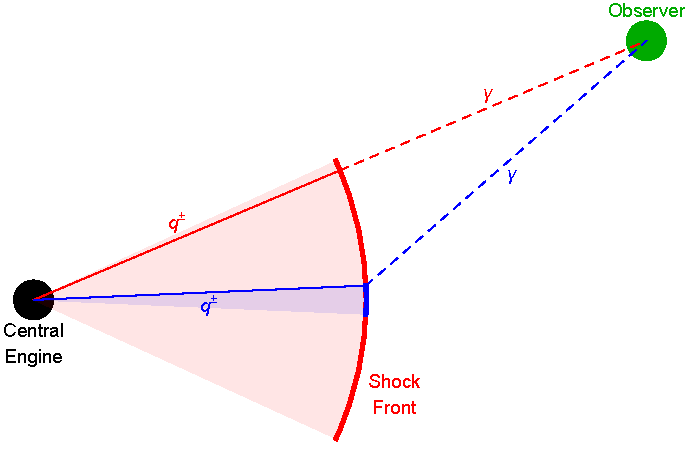
\includegraphics[width=0.7\textwidth]{modelOverview}
        \caption{ Model Overview.  The red and blue cones represent
          the regions through which low and high energy charged
          particles propagate.  In the case shown the observer's
          off-axis angle is smaller than the opening angle of the low
          energy jet, so, due to the relativistic beaming effect, the
          most of the observable low energy photons will travel along
          the straight line from the central engine.  Also, the
          observer's off-axis angle is larger that the opening angle
          of the high energy jet, but the high energy radiation will
          still originate near the center of the jet as this is the
          only place where the high energy radiators are located.  The
          observation time of a photon is a sum of two terms. First, the
          time interval spent in plasma as a radiator which
          approximately equals to the distance from the central engine
          to the point of emission. Second, the time interval from
          emission to detection which equals to the distance from the point
          of emission to the observer's location.  For the given position
          of the observer the sum is larger for high energy
          photons.  Therefore, the high energy emission will be
          observed later throughout the burst duration and the
          high energy light curve will be stretched.  }
        \label{fig:modelOverview}
	\end{figure}

	\begin{figure}
		\centering
		\hspace*{\fill}
		\begin{subfigure}{0.45\textwidth}
			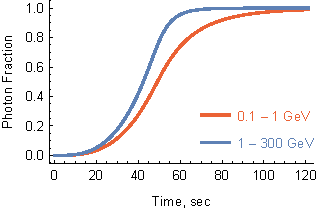
\includegraphics[width=\textwidth]{sampleLightCurveLogNegative}
			\label{fig:sampleLightCurveLogNegative}
			\caption{Stretching factor $\kappa = 0.819$, redshift $z = 1.82$, off-axis angle $\chi = 0$.}
		\end{subfigure}
		\hfill
		\begin{subfigure}{0.45\textwidth}
			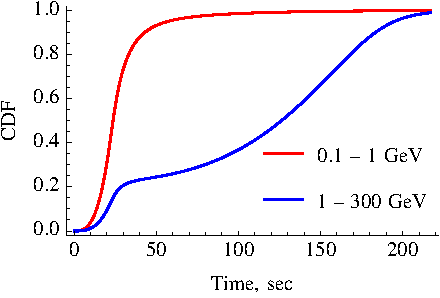
\includegraphics[width=\textwidth]{sampleLightCurveLogPositive}
			\label{fig:sampleLightCurveLogPosivie}
			\caption{Stretching factor $\kappa = 2.43$, redshift $z = 2.106$, off-axis angle $\chi = 5.90 \times 10^{-3}$.}
		\end{subfigure}
		\hspace*{\fill}
		\caption{
			High and low energy light curves produced by the geometrical model.
			Burst parameter values are the same as discussed in section \ref{sec:parameters}.
		}
		\label{fig:sampleLightCurves}
	\end{figure}

The basic idea of the model is illustrated in Figure
\ref{fig:modelOverview}. The model explains both the stretching
factors lower and higher than 1 with the difference of the position of
the observer with respect to the burst. The sample light curves are
shown in Figure \ref{fig:sampleLightCurves}. The detailed calculations
show that the stretching factors of GRB 090902B and GRB 090926A appear
naturally in the model. The predicted distribution of stretching
factors is shown in Figure \ref{fig:kappaDistribution}.

The rest of the paper is organized as follows. We describe the Fermi
LAT data and the analysis procedures in Section
\ref{sec:observations}. The model and the details on calculations are
explained in Section \ref{sec:model}. The Section \label{sec:tests}
introduces three phenomenological tests for the model. The parameters
of the model and the new method for estimating the jet observation
angles are shown in Section \ref{sec:results}. The code for modeling
is open source and is publicly available on GitHub
(\url{https://github.com/maxitg/GammaRays}).

\section{Data analysis}
\label{sec:observations}

\subsection{Fermi LAT Photon Selection}
\label{sec:photonSelection}

\begin{table}
	\centering
	\small
	\begin{tabular}{ l | S[table-format=9.3] | S[table-format=3.3] | S[table-format=-2.3] | S[table-format=1.5] | S[table-format=2.1] | S[table-format=3.1] }
		\multicolumn{1}{ c |}{GRB} & $\mathrm{GBM\ Trigger\ Time}$ & $\mathrm{R.A.}$ & $\mathrm{Dec.}$ & $\mathrm{Location\ Error}$ & $T_{05}$ & $T_{95}$ \\
		\multicolumn{1}{ c |}{Name}& $\mathrm{MET,\ sec}$ & $\mathrm{J2000,\ deg}$ & $\mathrm{J2000,\ deg}$ & $\mathrm{deg}$ & $\mathrm{sec}$ & $\mathrm{sec}$ \\
		\multicolumn{1}{ c |}{\texttt{name}} & $\mathrm{\texttt{time}}$ & \texttt{location.ra} & \texttt{location.dec} & \texttt{location.err} & \texttt{startOffset} & \texttt{endOffset} \\
		\hline
		080825C	&	241366429.105	&	233.9  	&	 -4.5  	&	0.75   	&	 3.2	&	 29.4	\\
		080916C	&	243216766.614	&	119.85 	&	-56.64 	&	0.0001 	&	 5.0	&	209.8	\\
		081006 	&	244996175.173	&	136.32 	&	-62.05 	&	0.52   	&	 0.7	&	115.0	\\
		081024B	&	246576161.864	&	322.95 	&	 21.2  	&	0.22   	&	 0.1	&	191.0	\\
		090217 	&	256539404.560	&	204.83 	&	 -8.42 	&	0.35   	&	 6.2	&	 68.0	\\
		090323 	&	259459364.630	&	190.71 	&	 17.053	&	0.0001 	&	15.9	&	293.9	\\
		090328 	&	259925808.510	&	 90.67 	&	-41.715	&	0.0002 	&	18.8	&	652.9	\\
		090510 	&	263607781.971	&	333.55 	&	-26.583	&	0.0004 	&	 0.6	&	 45.6	\\
		090626 	&	267683530.880	&	170.03 	&	-33.49 	&	0.22   	&	52.2	&	299.9	\\
		090902B	&	273582310.313	&	264.94 	&	 27.324	&	0.001  	&	 7.7	&	825.0	\\
		090926A	&	275631628.990	&	353.4  	&	-66.32 	&	0.01   	&	 5.5	&	225.0	\\
		091003 	&	276237347.585	&	251.52 	&	 36.625	&	0.0005 	&	 3.9	&	452.6	\\
		091031 	&	278683230.850	&	 71.49 	&	-57.65 	&	0.23   	&	 3.1	&	206.2	\\
		100116A	&	285370262.240	&	305.01 	&	 14.43 	&	0.17   	&	 3.0	&	141.0	\\
		100414A	&	292904423.990	&	192.11 	&	  8.693	&	0.0005 	&	17.4	&	288.6	\\
		110120A	&	317231981.230	&	 61.5  	&	-12.0  	&	0.36   	&	 0.5	&	112.8	\\
		110428A	&	325675112.410	&	  5.59 	&	 64.849	&	0.00001	&	10.7	&	407.6	\\
		110721A	&	332916465.760	&	333.2  	&	-38.5  	&	0.20   	&	 0.1	&	239.0	\\
		110731A	&	333803371.954	&	280.504	&	-28.537	&	0.0001 	&	 3.0	&	 24.1
	\end{tabular}
	\caption{Burst data used in our study taken from~\cite{Ackermann:2013zfa}. The third row contains
          the corresponding \texttt{GRBurst} class variable names of
          the software package \url{https://github.com/maxitg/GammaRays/blob/master/GRObservations/bursts}}
	\label{tab:bursts}
\end{table}

First, we download the Pass 7REP (V15) ``SOURCE'' class photons from
the Fermi-LAT data
server~\cite{2009ApJ...697.1071A,Ackermann:2012kna}. In order to
define the regions of interest we use the catalog
\cite{Ackermann:2013zfa}, which contains all the bright gamma-ray
bursts seen by the Fermi LAT since 2008 August 4 to 2011 August 1.
Specifically, we take 4 pieces of information from the tables 2 and 4
of Ref. \cite{Ackermann:2013zfa}:
\begin{itemize}
	\item{
		GBM trigger time.
		It is used as a reference point for the GRB time.
	}
	\item{
		Location of the GRB.
		The burst locations are used to filter out photons
                coming from the other sources.
	}
	\item{
		Location error.
		Location errors are used to improve the accuracy of filtering, specifically to avoid losing statistics by filtering too much.
	}
	\item{
		$T_{05}$ -- $T_{95}$ interval of the LAT-detected
          emission. The beginning of the interval is used as a fixed
          point of stretching. The Fermi LAT photons are downloaded
          for the period extended in time by $50\%$ towards both past
          and future compared to this interval.
	}
\end{itemize}
The data are summarized in table \ref{tab:bursts}. For the background
estimation, we also download observational data for 24 hours before
the burst.  The analysis is performed with the Fermi Science Tools
v9r32p5
package~\footnote{\url{http://fermi.gsfc.nasa.gov/ssc/data/analysis/scitools/overview.html}}
following the
guidelines~\footnote{\url{http://fermi.gsfc.nasa.gov/ssc/data/analysis/scitools/data_preparation.html}}.
We require Earth zenith angle to be below $100^\circ$ to remove the
Earth limb emission. After the basic filtering by \texttt{gtselect}
and \texttt{gtmktime} tools is done we perform more elaborate
selection using the point spread function of Fermi LAT, calculated
with \texttt{gtpsf} tool. We use 300 energy bins from \unit[100]{MeV}
to \unit[300]{GeV}, and 300 angular bins with maximal angle being
$30\degree$.  The \texttt{gtltcube} tool is used to compute required
livetime maps. Note, that we calculate PSFs separately for both
conversion types: front and back. We define $\mathrm{PSF}_{95}$ as an
angular distance from the source containing 95\% of the emitted
photons. We require that the photon is closer than $\mathrm{PSF}_{95}
+ \texttt{location.err}$ to the location of the GRB (see Table
\ref{tab:bursts}). The details of the data request and
analysis are given in appendix \ref{sec:fermiCode}.

%To understand how to use obtained PSFs, imagine a stream of photons
%coming from some source located at some coordinates $\theta,
%\phi$. Ideally, all the coordinates measured for the photons coming
%from the source should be the same. However, due to measurement
%errors, they would be spread across some region of the sky. If we find
%the region such that, say, $95\%$ of photons coming from the source
%are measured inside of it, we can filter out all the other photons
%without losing too much statistics, and significantly reducing
%background. \texttt{gtpsf} approximates these regions as circles, and
%the files generated in the previous step contain the observation
%probability densities as functions of distance from the source and
%photon energies. We, however, need an integral quantity, that is given
%the radius, we want to know the fraction of photons observed inside
%the circle of this radius. We can compute this fraction by summing
%over the probability densities:
%\begin{align*}
%	p\left(n\right) &= \int_0^n \texttt{pdf[i]} 2\pi \sin\left(\texttt{angles[i]}\right) \dif i \\
%	&\approx \sum_{i=0}^{n} \frac{\texttt{pdf[i]} + \texttt{pdf[i+1]}}{2} 2\pi \left(\cos\left(\texttt{angles[i]}\right) - \cos\left(\texttt{angles[i+1]}\right)\right)
%\end{align*}
%Here \texttt{pdf[i]} is the probability density in the point separated from the source by an angle \texttt{angles[i]}. And $p\left(n\right)$ is the probability to observe a photon closer to the source than \texttt{angles[n]}. We find probabilities for intermediate angles by linear interpolation. Finally, we can compute the inverse value $\theta_{\text{spread}}\left(p\right)$ (that is a distance as a function of probability) by binary search. Note, that $\theta_{\text{spread}}\left(p\right)$ depends on the photon energy, event class, and conversion type. We should use the appropriate function for each photon. The spread angles for intermediate energies are linearly interpolated.

The set will be used for the analysis with the reservation that it
unavoidably contains some background photons. We consider the
background flux constant in time and estimate it using the data for 24
hours before the burst. In order to calculate the number of background
photons we need an exposure map, which will be discussed in the
following section.

\subsection{Exposure Maps and Background Estimation}

The exposure map is computed with the \texttt{gtexpcube2} tool. We
compute it with 300 energy bins from \unit[100]{MeV} to
\unit[300]{GeV}. The produced \texttt{expcube} files contain exposures
as functions of energy and location on the sky. We use trilinear
interpolation to compute exposures for all energies and
locations. Knowing the exposures, we use the method introduced in the
appendix of \cite{Rubtsov:2011qq} to estimate the background for low
and high-energy bands. Note, that the ``TRANSIENT'' class photons are
not included in the analysis due to the strong dependence of the
background on the spacecraft position.

\subsection{KS-test}

Before applying the KS-test we subtract the background, which is
considered linear for the duration of the burst :

\begin{equation}
	\Phi_i\left(t\right) = \frac{p_i\left(T_1, t\right) - b_i \frac{t-T_1}{T_2-T_1}}{p_i\left(T_1, T_2\right) - b_i}
\end{equation}
Here $\left(T_1, T_2\right)$ is the time range of observations,
$p_i\left(t_1, t_2\right)$ is the number of photons observed in the
time range $t_1$ to $t_2$ in the $i$'s energy band ($i$ is either low
or high for the low and high-energy bands respectively), and $b_i$ is
the estimated number of background photons for the time range $T_1$ to
$T_2$ in the $i$'s energy band.

The number of degrees of freedom used as an input for the KS-test is
$p_i\left(T_1, T_2\right) - b_i$. This is lower than the number of
independent photons and therefore we are conservative when estimating
the probability and significance of the effect. The KS-probabilities
are computed for pairs $\Phi_\text{low}\left(t\right),
\Phi_\text{high}\left(\kappa t\right)$ to obtain the allowed ranges
for stretching factors $\kappa$ for a given confidence level.
% We evaluate stretching factors in the
%range $\texttt{STRETCHING\_MIN} = 0.1$ to $\texttt{STRETCHING\_MAX} =
%10.$ with a logarithmic step of $\texttt{STRETCHING\_STEP} = 1.001$.

\subsection{Stretching factors}

Out of 19 bursts studied, only 4 have at least 10 high energy events
remaining after the filtering, and thus eligible for computating the
stretching factors. The results of this computation are shown in
Figures \ref{fig:grb080916C}, \ref{fig:grb090510},
\ref{fig:grb090902B}, \ref{fig:grb090926A} and table
\ref{tab:observationResults}.

Out of these 4 bursts, two (GRB 080916C and GRB 090510) have
stretching factors compatible with $\kappa = 1$ within $2\sigma$
range.

GRB 090926A has, however, high energy radiation stretched with respect
to low energy radiation (that is $\kappa > 1$). In contrast to that,
GRB 090902B has low energy radiation stretched with respect to high
energy radiation ($\kappa < 1$).

Therefore we obtained an indication that the stretching factors for
observable bursts may take values both larger and smaller than $1$.

\begin{figure}
        \centering
        \begin{subfigure}{0.49\textwidth}
                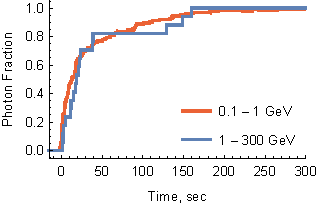
\includegraphics[width=\textwidth]{lightCurve080916C}
                \label{fig:lightCurve080916C}
        \end{subfigure}
        \begin{subfigure}{0.49\textwidth}
                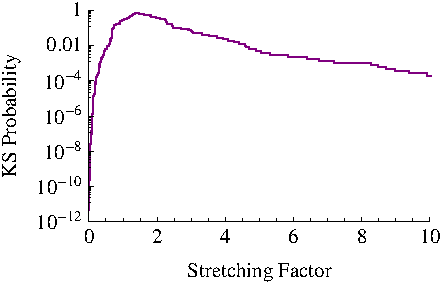
\includegraphics[width=\textwidth]{probabilities080916C}
                \label{fig:probabilities080916C}
        \end{subfigure}
        \caption{GRB 080916C light curves. Stretching factor is compatible with $\kappa = 1$ within $2\sigma$.}
        \label{fig:grb080916C}
\end{figure}

\begin{figure}
        \centering
        \begin{subfigure}{0.49\textwidth}
                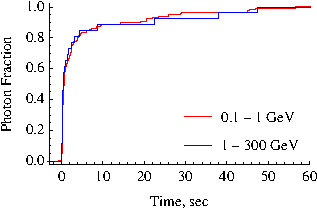
\includegraphics[width=\textwidth]{lightCurve090510}
                \label{fig:lightCurve090510}
        \end{subfigure}
        \begin{subfigure}{0.49\textwidth}
                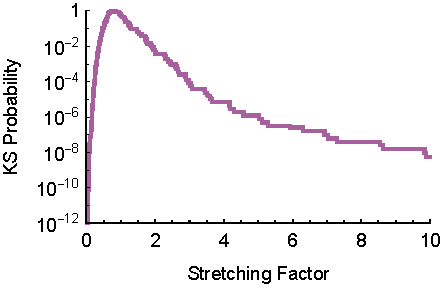
\includegraphics[width=\textwidth]{probabilities090510}
                \label{fig:probabilities090510}
        \end{subfigure}
        \caption{GRB 090510 light curves. Stretching factor is compatible with $\kappa = 1$ within $1\sigma$.}
        \label{fig:grb090510}
\end{figure}

\begin{figure}
        \centering
        \begin{subfigure}{0.49\textwidth}
                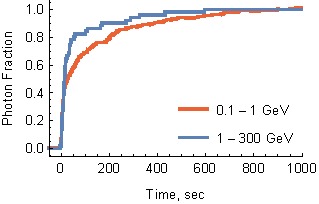
\includegraphics[width=\textwidth]{lightCurve090902B}
                \label{fig:lightCurve090902B}
        \end{subfigure}
        \begin{subfigure}{0.49\textwidth}
                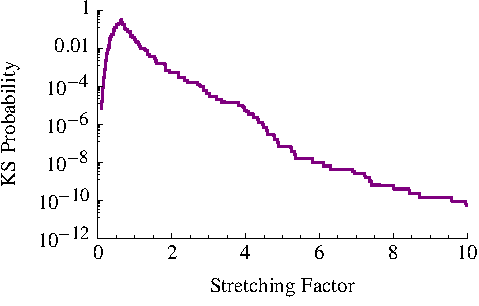
\includegraphics[width=\textwidth]{probabilities090902B}
                \label{fig:probabilities090902B}
        \end{subfigure}
        \caption{GRB 090902B light curves. Low energy radiation is stretched ($\kappa < 1$) with significance of $2.3\sigma$.}
        \label{fig:grb090902B}
\end{figure}

\begin{figure}
        \centering
        \begin{subfigure}{0.49\textwidth}
                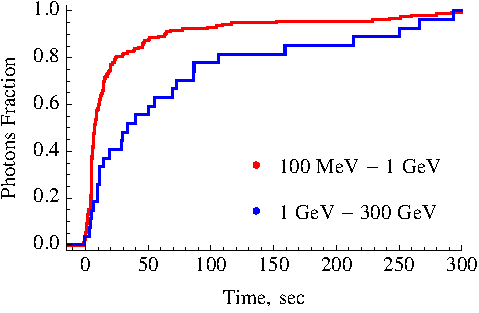
\includegraphics[width=\textwidth]{lightCurve090926A}
                \label{fig:lightCurve090926A}
        \end{subfigure}
        \begin{subfigure}{0.49\textwidth}
                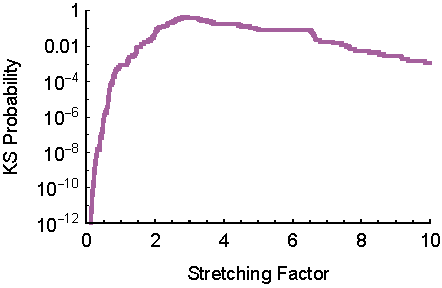
\includegraphics[width=\textwidth]{probabilities090926A}
                \label{fig:probabilities090926A}
        \end{subfigure}
        \caption{GRB 090926A light curves. High energy radiation is stretched ($\kappa > 1$) with significance of $3.3\sigma$.}
        \label{fig:grb090926A}
\end{figure}

\begin{table}
	\centering
	\small
	\begin{tabular}{ l | S[table-format=2.3]@{\; -- \;}S[table-format=2.3] | S[table-format=2.3]@{\; -- \;}S[table-format=2.3] | S[table-format=2.3]@{\; -- \;}S[table-format=2.3] | S[table-format=2.3]@{\; -- \;}S[table-format=2.3] | S[table-format=2.3]@{\; -- \;}S[table-format=2.3] }
		\multicolumn{1}{ c |}{GRB} & \multicolumn{2}{ c |}{$1\sigma$} & \multicolumn{2}{ c |}{$2\sigma$} & \multicolumn{2}{ c |}{$3\sigma$} & \multicolumn{2}{ c |}{$4\sigma$} & \multicolumn{2}{ c }{$5\sigma$} \\
		\hline
		080916C	&	1.04  & 2.24	&	0.67 & 3.32	&	0.42 & 5.83	&	0.19 & 14.9		&	0.087 & 35.7	\\
		090501	&	0.58  & 1.1		&	0.43 & 1.61	&	0.32 & 2.29	&	0.22 &  3.03	&	0.17  &  5.11	\\
		090902B	&	0.604 & 0.613	&	0.35 & 0.89	&	0.22 & 1.53	&	0.13 &  2.86	&	0.078 &  4.49	\\
		090926A &	2.61  & 3.33	&	1.99 & 6.62	&	1.34 & 9.15	&	0.73 & 13.5		&	0.48  & 19.4
	\end{tabular}
	\caption{The ranges of allowed stretching factors for multiple
          levels of significance for the GRBs studied.}
	\label{tab:observationResults}
\end{table}


\section{Model}
\label{sec:model}

The main idea behind our model is to assume that the burst opening angle depends on energy of emitted photons, or, equivalently, that the most energetic plasma particles are concentrated near the axis of the jet, while low energy particles are on the periphery.
As you can see in Figure \ref{fig:modelOverview} this leads to a time stretching effect in some cases due to relativistic beaming.

At the moment, we do not have any rigorous proof of our assumption.
There are arguments, however, supporting it.

First of all, the number of observed GRBs rapidly decreases with energy.
There are around 750 bursts detected by GBM in hard X-rays and low
energy gamma rays \cite{Vianello:2013ela} (half of them were in a LAT
field of view), only 30 or so were detected by LAT above
\unit[100]{MeV}, and only about 4 of them were detected above GeV.

% TODO merge 2
First of all, the number of observed GRBs rapidly decreases with energy.
There are around 750 bursts detected by GBM in hard X-rays and low
energy gamma rays \cite{Vianello:2013ela} (half of them were in a LAT
field of view), only 30 or so were detected by LAT above
\unit[100]{MeV}, and only about 4 of them were detected above GeV.


First of all, there are around 750 GRBs detected by GBM, half of which
were in the LAT field of view at the moment of observation
\cite{Vianello:2013ela}.  However, only about 30 of them were detected
by the LAT, and only 4 of them were bright in the high energy band.
If we extrapolate the uniform jet model to very high energies, this
observation would mean that these groups of bursts are internally
different: some of them produce VHE radiation, while others do not.
These differences are hard to explain given that burst energetics are
similar \cite{Bloom:2003wy}.  Nevertheless, these differences in burst
counts can easily be explained by our model.  In our model, the
opening angle of a jet is inversely proportional to the energy of
photons it radiates.  Therefore the most common scenario is that the
off-axis angle of an observer is smaller than the low energy jet
opening angle, but much larger than the opening angle of a high energy
jet.  Because of that, most of the bursts can only be seen at low
energies.  The 4 bursts we study in this paper were seen, according to
our model, from the lowest off-axis angles.


This observation is hard to explain in a framework of uniform jet model given that burst energetics are similar \cite{Bloom:2003wy}.
It is, however, easy to explain in our model, given that small observation angles are rare, and the only way to produce high energy radiation is to have the observation angle small enough.

% merge 
Another argument comes from consideration of processes happening in
jets, specifically the scattering of particles near the jet boundary.
While plasma particles scatter, they simultaneously lose energy, and
change directions, sometimes propagating beyond the jet boundary, and
therefore increasing the jet opening angle.  So, the processes of
energy loss and increase of jet size are correlated, therefore the low
energy particles should be closer to the jet boundary.

Second, consider the plasma right after its ejection from the central
engine.  Two processes happen there simultaneously:
\begin{enumerate}
	\item{Particles near the jet boundary collide and change their
          movement directions, therefore increasing the opening angle
          of the jet.}
	\item{Particles lose energy, therefore decreasing radiation
          frequency emitted by the jet.}
\end{enumerate}
We argue that these two processes are correlated, for they happen due
to the same particle interaction processes.  And since they are
correlated, jets with larger opening angles should have lower
energies, which is the assumption we are trying to justify.


In the following sections we will rigorously derive the procedure for computing time stretching factors from our model, and compare them to observations obtained in the previous section.

To understand the observed spectral lag, lets explore geometry of the jet. First of all, lets make some assumptions:
\begin{enumerate}
\item{Time $t = 0$, a spherical shell of plasma is emitted. The center is called the central engine.}
\item{The shell points propagate with a constant velocity $v = \frac{\sqrt{\gamma^2 - 1}}{\gamma} \sim 1$, so at the time $t$ the radius of the shall is $v t$.}
\item{Each point of the shell is an isotropic radiator in its rest frame.}
\item{
	The radiation intensity is a function of the radiator position and the radiation frequency:
	\begin{equation}
		\eta\left(r,\theta,\omega\right) = 
		\frac{\eta_0}{1 + \left(\frac{r}{r_0}\right)^n}
		\exp\left(
			-\left(\frac{\theta}{\theta_0}\right)^2
			\left(\frac{\omega}{\omega_0}\right)^{-2k}
		\right)
		\left(\frac{\omega}{\omega_0}\right)^\alpha
	\end{equation}
	$\eta$ is a number of particles emitted per volume per solid angle per frequency. It is a function of the distance $r$ from the central engine, of the off-axis angle $\theta$, and of the radiation frequency $\omega$.
}
\end{enumerate}

The burst is fully specified by the following set of parameters:
\begin{itemize}
\item{$\gamma$, the relativistic factor of the shell, $\gamma \gg 1$.}
\item{$\eta_0$, which defines the luminosity scale.}
\item{$r_0$, the characteristic jet length; $r_0 \ll \frac{1}{H\left(0\right)}$, $H\left(t\right)$ is the Hubble parameter;}
\item{$n$, which determines the sharpness of the jet end, $n > 3$;}
\item{$\omega_0$, a characteristic radiation frequency;}
\item{$\theta_0$, the opening angle of the jet for radiation with frequency $\omega_0$, $\theta_0 \ll 1$;}
\item{$k$, which determines how much the opening angle changes with frequency, $k < 0$;}
\item{$\alpha$, the bare spectral index, $\alpha < -2k - 1$}
\end{itemize}

Now we have all we need to calculate the observed light curves, and then the stretching factors.

\subsection{Photon observation time}

Lets begin by computing a time at which some particular photon is observed. This time is a function of the radiator location $\left(r, \theta, \phi\right)$, as well as the observer location $\left(d, \chi, 0\right)$. (Here we choose coordinates so that the rotation angle of the observer is $0$.) Lets assume for now that the observer is too far from the jet to resolve its geometry, yet close enough so that the expansion of space is negligible. This assumption allows us to ignore the effects of cosmology for this calculation.

The observation time is a sum of two terms: the time interval from $t = 0$ to the photon emission (the plasma time), and the time interval between the emission and the observation (the photon time):
\begin{equation*}
t\left(r, \theta, \phi, d, \chi\right) = t_\text{plasma}\left(r\right) + t_\text{photon}\left(r, \theta, \phi, d, \chi\right)
\end{equation*}
$t_\text{plasma}$ is easy to compute since plasma moves with uniform velocity:
\begin{equation*}
t_\text{plasma}\left(r\right) = \frac{r}{v}
\end{equation*}
$t_\text{photon}$ is a distance between the radiator and the observer:
\begin{align*}
t_\text{photon}\left(r, \theta, \phi, d, \chi\right) &= \sqrt{
	\left( d \cos\chi - r \cos\theta \right)^2 +
	\left( d \sin\chi - r \sin\theta \cos\phi \right)^2 +
	\left( r \sin\theta \sin\phi \right)^2
} \\
&= d\sqrt{
	\left( \cos\chi - \frac{r}{d} \cos\theta \right)^2 +
	\left( \sin\chi - \frac{r}{d} \sin\theta \cos\phi \right)^2 +
	\left(\frac{r}{d} \sin\theta \sin\phi \right)^2
} \\
&\sim d\sqrt{
	\cos^2{\chi} - 2\frac{r}{d} \cos\theta \cos\chi + \sin^2\chi - 2\frac{r}{d} \sin\theta \cos\phi \sin\chi
} \\
&\sim d\left(
	1 - 
	\frac{r}{d} \left( \cos\theta \cos\chi + \sin\theta \cos\phi \sin\chi \right)
\right) \\
&= d - r\left( \cos\theta \cos\chi + \sin\theta \cos\phi \sin\chi \right)
\end{align*}
Combining these expressions together, we get:
\begin{equation*}
t\left(r, \theta, \phi, d, \chi\right) = d + r\left( \frac{1}{v} - \cos\theta \cos\chi - \sin\theta \cos\phi \sin\chi \right)
\end{equation*}
Since no photon can reach the observer faster than the speed of light, and the photons emitted at $t = 0$ reach the observer at $t = d$, this time $t = d$ is the start of the observer's light curve. So we can define a more convenient time origin:
\begin{equation*}
\tau \left(r, \theta, \phi, \chi\right) = t\left(r, \theta, \phi, d, \chi\right) - d = r\left( \frac{1}{v} - \cos\theta \cos\chi - \sin\theta \cos\phi \sin\chi \right)
\end{equation*}
Finally, we can use the spherical law of cosines to write this in terms of the great-circle distance $\sigma\left( \theta, \phi, \chi \right)$ between the points $\left( \theta, \phi \right)$ and $\left( \chi, 0 \right)$:
\begin{equation}
\tau \left(r, \theta, \phi, \chi\right) = r\left( \frac{1}{v} - \cos\sigma\left( \theta, \phi, \chi \right) \right)
\end{equation}

Note that $\tau$ doesn't depend on $d$ anymore. But this is only true if we did not account for cosmology, or if the scale factor did not change from emission to observation. For a distant observer it will change, however, which will stretch the distances between photons:
\begin{equation}
\tau \left(r, \theta, \phi, z, \chi \right) = r\left( \frac{1}{v} - \cos\sigma\left( \theta, \phi, \chi \right) \right) \left( 1 + z \right)
\end{equation}
Here $z$ is the redshift of the burst from the point of view of the observer.

\subsection{Light curve}
We now know enough to compute the observable quantity - the number of observed photons $p$. For that we need to integrate the radiation intensity $\eta$ over four things. Two burst-related things: radiator positions $\left(r, \theta, \phi\right)$ and frequencies at emission $\omega'$. Two observer-related things: observation time $\tau$ and frequencies at observation $\omega$. We relate the first two and the second two with the delta functions:
\begin{align}
p\left( z, \chi; \tau_1, \tau_2; \omega_1, \omega_2 \right) &= \frac{A_\text{det}}{A_\text{ph}\left(z\right)} \int_0^\infty \dif r \int_0^{\pi} r \dif \theta \int_0^{2\pi} r \sin{\theta} \dif \phi \int_0^\infty \dif \omega' \int_{\tau_1}^{\tau_2} \dif \tau \int_{\omega_1}^{\omega_2} \dif \omega \, \eta\left( r, \theta, \omega' \right) \nonumber\\
&\qquad {} \times \underbrace{\frac{1}{\gamma^2\left( 1 - v \cos\sigma\left(\theta, \phi, \chi\right) \right)^2}}_{\text{aberration}} \underbrace{\frac{1}{\gamma\left( 1 - v \cos\sigma\left(\theta, \phi, \chi\right) \right)}}_{\text{time dilation}} \nonumber\\
&\qquad {} \times \delta\left( \frac{\omega'}{\underbrace{\gamma \left( 1 - v\cos\sigma\left(\theta, \phi, \chi\right) \right)}_{\text{relativistic shift}} \underbrace{\left(1+z\right)}_{\text{cosmological shift}}} - \omega \right) \nonumber\\
&\qquad {} \times \delta\left( \tau - r\left( \frac{1}{v} - \cos\sigma\left(\theta, \phi, \chi\right) \right) \left(1+z\right) \right)
\end{align}
Here $A_\text{det}$ is the effective area of the detector, and $A_\text{ph}$ is an area of the sphere over which photons emitted in the burst are spread (see appendix \ref{sec:cosmology} for derivation). We have taken account for four relativistic effects, which affect intensities and frequencies of the radiators: relativistic aberration; time dilation of the radiators relative to the observer; relativistic blue/redshift; and cosmological redshift.

We can use the delta functions to do the integrals over $\omega'$ and $r$. For that lets transform the first one:
\begin{align*}
\delta\left( \frac{\omega'}{\gamma \left( 1 - v\cos\sigma \right)\left(1+z\right)} - \omega \right) &= \delta\left( \frac{1}{\gamma\left( 1-v\cos\sigma \right)\left(1+z\right)} \left( \omega' - \gamma\left( 1 - v\cos\sigma \right) \left(1+z\right) \omega \right) \right) \\
&= \gamma\left( 1 - v\cos\sigma \right) \left(1+z\right) \delta\left( \omega' - \gamma\left( 1 - v\cos\sigma \right) \left(1+z\right) \omega \right)
\end{align*}
And the second one:
\begin{align*}
\delta\left(\tau - r\left( \frac{1}{v} - \cos\sigma \right)\left(1+z\right)\right) &= \delta\left( \left( \frac{1}{v} - \cos\sigma \right) \left( 1+z \right) \left( r - \frac{\tau}{\left(\frac{1}{v} - \cos\sigma\right)\left(1+z\right)} \right) \right) \\
&= \frac{1}{\left(\frac{1}{v} - \cos\sigma\right)\left(1+z\right)} \delta\left( r - \frac{\tau}{\left(\frac{1}{v} - \cos\sigma\right)\left(1+z\right)} \right)
\end{align*}
After the transformations expression for $p$ takes the following form:
\begin{align}
p\left( z, \chi; \tau_1, \tau_2; \omega_1, \omega_2 \right) &= \frac{A_\text{det}}{A_\text{ph}\left(z\right)} \int_0^{\pi} \dif \theta \int_0^{2\pi} \dif \phi \int_{\tau_1}^{\tau_2} \dif \tau \int_{\omega_1}^{\omega_2} \dif \omega \nonumber\\
&\qquad {} \times \eta\left( \frac{\tau}{\left(\frac{1}{v} - \cos\sigma\left(\theta, \phi, \chi\right)\right)\left(1+z\right)}, \theta, \gamma\left( 1 - v\cos\sigma\left(\theta, \phi, \chi\right) \right)\left(1+z\right)\omega  \right) \nonumber\\
&\qquad {} \times \frac{\tau^2 \sin\theta}{\left(\frac{1}{v} - \cos\sigma\left(\theta, \phi, \chi\right)\right)^3 \left(1+z\right)^2 \gamma^2 \left(1-v\cos\sigma\left(\theta, \phi, \chi\right)\right)^2} \nonumber\\
&= \frac{A_\text{det}}{A_\text{ph}\left(z\right)} \frac{1}{v^2 \gamma^2 \left(1+z\right)^2} \int_{\tau_1}^{\tau_2} \dif \tau \, \tau^2 \int_0^{\frac{\pi}{2}} \dif \theta \int_0^{2\pi} \dif \phi \int_{\omega_1}^{\omega_2} \dif \omega \frac{\sin\theta}{\left(\frac{1}{v} - \cos\sigma\left(\theta, \phi, \chi\right)\right)^5} \nonumber\\
&\qquad {} \times \eta\left( \frac{\tau}{\left(\frac{1}{v} - \cos\sigma\left(\theta, \phi, \chi\right)\right)\left(1+z\right)}, \theta, \gamma\left( 1 - v\cos\sigma\left(\theta, \phi, \chi\right) \right)\left(1+z\right)\omega  \right)
\end{align}

Furthermore, if we write $\eta$ explicitly we can do the integrals over $\omega$ and $\tau$:
\begin{align}
p\left( z, \chi; \tau_1, \tau_2; \omega_1, \omega_2 \right) &= \frac{A_\text{det}}{A_\text{ph}\left(z\right)} \frac{1}{v^2 \gamma^2 \left(1+z\right)^2} \int_0^{\pi} \dif \theta \int_0^{2\pi} \dif \phi \int_{\omega_1}^{\omega_2} \dif \omega \int_{\tau_1}^{\tau_2} \dif \tau \, \tau^2 \frac{\sin\theta}{\left(\frac{1}{v} - \cos\sigma\left(\theta, \phi, \chi\right)\right)^5} \nonumber\\
&\qquad {} \times \frac{\eta_0}{1 + \left(\frac{\tau}{r_0\left(\frac{1}{v} - \cos\sigma\left(\theta, \phi, \chi\right)\right)\left(1+z\right)}\right)^n} \nonumber\\
&\qquad {} \times \exp\left(
	-\left(\frac{\theta}{\theta_0}\right)^2
	\left(\frac{\omega\gamma\left( 1 - v\cos\sigma\left(\theta, \phi, \chi\right) \right)\left(1+z\right)}{\omega_0}\right)^{-2k}
\right) \nonumber\\
&\qquad {} \times \left(\frac{\omega\gamma\left( 1 - v\cos\sigma\left(\theta, \phi, \chi\right) \right)\left(1+z\right)}{\omega_0}\right)^\alpha \nonumber\\
&= \frac{A_\text{det}}{A_\text{ph}\left(z\right)} \frac{\eta_0}{\left(v\gamma\left(1+z\right)\right)^{2-\alpha}} \int_0^{\pi} \dif \theta \int_0^{2\pi} \dif \phi \frac{\sin\theta}{\left(\frac{1}{v} - \cos\sigma\left(\theta, \phi, \chi\right)\right)^{5-\alpha}} \nonumber\\
&\qquad {} \times \int_{\omega_1}^{\omega_2} \dif \omega \exp\left(
	-\left(\frac{\theta}{\theta_0}\right)^2
	\left(\frac{\omega\gamma\left( 1 - v\cos\sigma\left(\theta, \phi, \chi\right) \right)\left(1+z\right)}{\omega_0}\right)^{-2k}
\right) \left(\frac{\omega}{\omega_0}\right)^\alpha \nonumber\\
&\qquad {} \times \int_{\tau_1}^{\tau_2} \dif \tau \, \tau^2 \frac{1}{1 + \left(\frac{\tau}{r_0\left(\frac{1}{v} - \cos\sigma\left(\theta, \phi, \chi\right)\right)\left(1+z\right)}\right)^n} \nonumber\\
&= \frac{A_\text{det}}{A_\text{ph}\left(z\right)}
\frac{\eta_0}{\left(v\gamma\left(1+z\right)\right)^{2-\alpha}}
\int_0^{\pi} \dif \theta \int_0^{2\pi} \dif \phi \frac{\sin\theta}{\left(\frac{1}{v} - \cos\sigma\left(\theta, \phi, \chi\right)\right)^{5-\alpha}} \nonumber\\
&\qquad {} \times \left( I\left(z,\chi,\omega_2; \theta,\phi\right) - I\left(z,\chi,\omega_1; \theta,\phi\right) \right) \left( J\left(z,\chi,\tau_2; \theta,\phi\right) - J\left( z,\chi,\tau_1; \theta,\phi \right) \right)
\end{align}
Here $I$ and $J$ are indefinite integrals over $\omega$ and $\tau$:
\begin{align}
I\left(z,\chi,\omega;\theta,\phi\right) &= \frac{
	\omega
	\left(\frac{\omega}{\omega_0}\right)^{\alpha }
	E_{\frac{\alpha +1}{2 k}+1}\left(
		\left(\frac{\theta}{\theta_0}\right)^2
		\left(\frac{\omega}{\omega_0}\right)^{-2k}
		\left(
			\gamma \left(1-v \cos \sigma\left(\theta ,\phi ,\chi \right) \right) \left(1+z\right)
		\right)^{-2 k}
	\right)
}{
	2 k
} \\
J\left(z,\chi,\tau;\theta,\phi\right) &= \frac{\tau^3}{3} \,
_2F_1\left(
	1,
	\frac{3}{n};
	\frac{n+3}{n};
	-\left(\frac{\tau}{
		r_0 \left( \frac{1}{v} - \cos\sigma\left( \theta,\phi,\chi \right) \right) \left(1+z\right)
	}\right)^n
\right)
\end{align}
where exponential integral function $E_n\left(x\right) = \int_1^\infty \frac{e^{-x t} \dif t}{t^n}$.

The remaining integrals over $\theta$ and $\chi$ are hard to do symbolically, so we compute them numerically. To optimize this computation we can use the assumption of small $\theta$ and $\chi$, so that:
\begin{align*}
\sin\theta &\sim \theta \\
\cos\sigma\left(\theta, \phi, \chi \right) &= \cos\theta \cos\chi + \sin\theta \sin\chi \cos\phi \sim 1 - \frac{\theta^2}{2} - \frac{\chi^2}{2} + \theta\chi\cos\phi
\end{align*}
Using this assumption, and the evenness of the integral as a function of $\theta$, we arrive to the optimized expressions for $p$, $I$ and $J$:
\begin{align}
\label{eq:p}
p\left( z, \chi; \tau_1, \tau_2; \omega_1, \omega_2 \right) &= \frac{A_\text{det}}{A_\text{ph}\left(z\right)}
\frac{2\eta_0}{\left(v\gamma\left(1+z\right)\right)^{2-\alpha}}
\int_0^{\infty} \dif \theta \int_0^{\pi} \dif \phi \frac{\theta}{\left(\frac{1}{v} - 1 + \frac{\theta^2}{2} + \frac{\chi^2}{2} - \theta\chi\cos\phi\right)^{5-\alpha}}\nonumber\\
&\qquad {} \times \left( I\left(z,\chi,\omega_2; \theta,\phi\right) - I\left(z,\chi,\omega_1; \theta,\phi\right) \right) \left( J\left(z,\chi,\tau_2; \theta,\phi\right) - J\left( z,\chi,\tau_1; \theta,\phi \right) \right) \\
I\left(z,\chi,\omega;\theta,\phi\right) &= \frac{
	\omega
	\left(\frac{\omega}{\omega_0}\right)^{\alpha }
	E_{\frac{\alpha +1}{2 k}+1}\left(
		\left(\frac{\theta}{\theta_0}\right)^2
		\left(\frac{\omega}{\omega_0}\right)^{-2 k}
		\left(
			v \gamma \left(1+z\right) \left(\frac{1}{v} - 1 + \frac{\theta^2}{2} + \frac{\chi^2}{2} - \theta\chi\cos\phi \right)
		\right)^{-2 k}
	\right)
}{
	2 k
} \\
J\left(z,\chi,\tau;\theta,\phi\right) &= \frac{\tau^3}{3} \,
_2F_1\left(
	1,
	\frac{3}{n};
	\frac{n+3}{n};
	-\left(\frac{\tau}{
		r_0 \left( \frac{1}{v} -  1 + \frac{\theta^2}{2} + \frac{\chi^2}{2} - \theta\chi\cos\phi \right) \left(1+z\right)
	}\right)^n
\right)
\end{align}

Finally, we will need to compute limits of $p$ for $\omega_2 \rightarrow \infty$ and $\tau_2 \rightarrow \infty$. It requires us to know the limit of $I$ for $\omega \rightarrow \infty$ (we assumed that $k < 0$):
\begin{equation}
I\left(z,\chi,\infty;\theta,\phi\right) = \lim_{\omega \rightarrow \infty} I\left(z,\chi,\omega;\theta,\phi\right) = 0
\end{equation}
and the limit of $J$ for $\tau \rightarrow \infty$ ($n > 3$ by assumption):
\begin{equation}
J\left(z,\chi,\infty;\theta,\phi\right) = \lim_{\tau \rightarrow \infty} J\left(z,\chi,\tau;\theta,\phi\right) = \left(r_0 \left( \frac{1}{v} -  1 + \frac{\theta^2}{2} + \frac{\chi^2}{2} - \theta\chi\cos\phi \right) \left(1+z\right)\right)^3 \frac{\pi}{n\sin\frac{3\pi}{n}}
\end{equation}

Now, when we know $p$, we can compute many different things with it. For example:
\begin{itemize}
\item{the total number of particles observed in a given energy range, $p_\infty\left(z,\chi; \omega_1,\omega_2\right) = p\left( z,\chi; 0,\infty; \omega_1,\omega_2 \right)$;}
\item{the fraction of photons observed during a given time interval, $\Phi\left(z,\chi; \tau_1,\tau_2; \omega_1,\omega_2\right) = \frac{p\left( z,\chi; \tau_1,\tau_2; \omega_1,\omega_2\right)}{p_\infty\left( z,\chi; \omega_1,\omega_2 \right)}$;}
\item{the duration of the burst $T_f\left( z,\chi;\omega_1,\omega_2 \right)$, that is the time by which the fraction $f$ of photons is observed. We can compute it by solving the following equation for $T_f$: $p\left( z,\chi; 0,T_f; \omega_1,\omega_2\right) = f p_\infty\left( z,\chi; \omega_1,\omega_2 \right)$;}
\item{the stretching factor, which we will discuss in the next section.}
\end{itemize}

\subsection{Stretching factor}
The stretching factor for a continuous light curve is defined exactly like the stretching factor for a discrete one. It is the value of $\kappa$ which makes the KS-distance minimal:
\begin{equation}
\kappa\left(z,\chi; \omega_1, \omega_2, \omega_3\right) = \argmin_\kappa \max_\tau\left| \Phi\left(z,\chi; 0,\tau; \omega_1,\omega_2\right) - \Phi\left( z,\chi; 0,\kappa \tau; \omega_2,\omega_3 \right) \right|
\end{equation}

The maximum of an absolute value cannot be differentiated, so the computation of $\kappa$ by the given definition is complicated. Lets instead rewrite this expression in terms of a positive and a negative KS-distances:
\begin{align*}
D_+\left(z,\chi; \kappa; \omega_1, \omega_2, \omega_3\right) &= \max_\tau\left( \Phi\left(z,\chi; 0,\tau; \omega_1,\omega_2\right) - \Phi\left( z,\chi; 0,\kappa \tau; \omega_2,\omega_3 \right) \right) \\
D_-\left(z,\chi; \kappa; \omega_1, \omega_2, \omega_3\right) &= \min_\tau\left( \Phi\left(z,\chi; 0,\tau; \omega_1,\omega_2\right) - \Phi\left( z,\chi; 0,\kappa \tau; \omega_2,\omega_3 \right) \right) \\
\kappa\left(z,\chi; \omega_1, \omega_2, \omega_3\right) &= \argmin_\kappa \max\left(D_+\left(z,\chi; \kappa; \omega_1, \omega_2, \omega_3\right), -D_-\left(z,\chi; \kappa; \omega_1, \omega_2, \omega_3\right)\right)
\end{align*}

Take note that $\Phi$ monotonously increases with $\tau$. It implies that $D_+$ and $D_-$ monotonously decrease with $\kappa$, so as $D_+ + D_-$. So there is a single value of $\kappa$, for which
\begin{equation}
D_+\left(z,\chi; \kappa; \omega_1, \omega_2, \omega_3\right) = -D_-\left(z,\chi; \kappa; \omega_1, \omega_2, \omega_3\right)
\end{equation}
And this value of $\kappa$ also makes the $\max\left({D_+, -D_-}\right)$ minimal, since $D_+$ monotonously decrease, and $\left(-D_-\right)$ monotonously increase with $\kappa$.

So we have now a simpler way to compute $\kappa$ by solving an equation instead of computing the minimum. And $\Phi$ can be differentiated, which makes it easier to compute maximums and minimums of their differences.

Being able to compute the stretching factor, we could now compare our model predictions with observations given the position of an observer. We don't know the observer's off-axis angle $\chi$, however, so we cannot check the stretching factor prediction directly. Instead, we will focus on a series of tests, which will ensure that our model doesn't contradict existing observations. These tests will be discussed in the following sections.


\section{Observational tests}
\label{sec:tests}
\subsection{Total energy}

The first test is to compute the total energy radiated from the burst, and to ensure that it doesn't exceed the mass of the star from which the burst originated.

To compute the total energy, we need to multiply the radiation intensity by frequency, and integrate it over frequencies $\omega$, volume $\left(r,\theta,\phi\right)$, and observer positions $\left(\sigma, \xi\right)$. We assumed $\theta \ll 1$, and have taken into account the same relativistic effects as we did in the observed particle count computation:
\begin{align}
E &= \int_0^\infty \dif \omega \int_0^\infty \dif r \int_0^\infty r \dif \theta \int_0^{2\pi} r \, \theta \dif \phi \int_0^\infty \dif \sigma \int_0^{2\pi} \sin\sigma \dif \xi \nonumber\\
&\quad {} \times \eta\left( r,\theta,\omega \right) \underbrace{\frac{1}{\gamma\left(1-v\cos\sigma \right)}}_{\text{time dilation}} \underbrace{\frac{1}{\gamma^2\left(1-v\cos\sigma \right)^2}}_{\text{aberration}} \underbrace{\frac{\omega}{\gamma\left(1-v\cos\sigma \right)}}_{\text{relativistic shift}} \\
&= \frac{4\pi^2}{\gamma^4} \int_0^\infty \dif \omega \, \omega \int_0^\infty \dif r \, r^2 \int_0^\infty \dif \theta \, \theta \, \eta\left( r,\theta,\omega \right) \int_0^\infty \dif \sigma \frac{\sin\sigma}{\left(1-v\cos\sigma \right)^4} \nonumber
\end{align}
An integral over $\sigma$ is computable analytically:
\begin{equation*}
\int_0^\infty \dif \sigma \frac{\sin\sigma}{\left(1-v\cos\sigma \right)^4} = \frac{2\left(3+v^2\right)}{3\left(1-v^2\right)^3} = \frac{2}{3}\gamma^6 \left(4 - \frac{1}{\gamma^2}\right)
\end{equation*}
Substituting this result into the expression for $E$ we get:
\begin{equation}
E = \frac{32\pi^2}{3}\left(\gamma^2 - \frac{1}{4}\right) \int_0^\infty \dif \omega \, \omega \int_0^\infty \dif r \, r^2 \int_0^\infty \dif \theta \, \theta \, \eta\left( r,\theta,\omega \right)
\end{equation}
Now we can use the expression for $\eta$ to do the remaining integrals:
\begin{align*}
E = \frac{32\pi^2 \eta_0}{3}\left(\gamma^2 - \frac{1}{4}\right) \int_0^\infty \dif \omega \, \omega \left(\frac{\omega}{\omega_0}\right)^\alpha \int_0^\infty \dif r \, \frac{r^2}{1 + \left(\frac{r}{r_0}\right)^n} \int_0^\infty \dif \theta \, \theta \, \exp\left(-\left(\frac{\theta}{\theta_0}\right)^2\left(\frac{\omega}{\omega_0}\right)^{-2k}\right)
\end{align*}
The integrals over $r$ and $\theta$ can be computed symbolically:
\begin{equation*}
\int_0^\infty \dif r \, \frac{r^2}{1 + \left(\frac{r}{r_0}\right)^n} = \frac{\pi}{n\sin\left(\frac{3\pi}{n}\right)}r_0^3
\end{equation*}
\begin{equation*}
\int_0^\infty \dif \theta \, \theta \, \exp\left(-\left(\frac{\theta}{\theta_0}\right)^2\left(\frac{\omega}{\omega_0}\right)^{-2k}\right) = \frac{1}{2}\theta_0^2 \left(\frac{\omega}{\omega_0}\right)^{2k}
\end{equation*}
Now we have only one integral left:
\begin{equation}
E = \frac{16\pi^3}{3 n\sin\left(\frac{3\pi}{n}\right)} \left(\gamma^2 - \frac{1}{4}\right) \, \eta_0 \, r_0^3 \, \theta_0^2 \int_0^\infty \dif \omega \, \omega \left(\frac{\omega}{\omega_0}\right)^{2k+\alpha}
\end{equation}

Note, however, that since $\alpha < -2k-1$ this integral diverges for $\omega \rightarrow 0$. But our model is not expected to describe low-energy radiation of the burst, so we should not integrate over low-frequency radiators. Nevertheless, we should ensure that the total energy of the high-energy radiation is not too large. To compute this energy we will only integrate over those radiators which emission we can observe, that is over the radiators with frequencies greater than $\frac{\omega_1}{\gamma}$, where $\omega_1$ is the smallest observable photon frequency. Now we can compute the last integral and get the final expression for $E$:
\begin{align}
E\left(\omega_1\right)
&= \frac{16\pi^3}{3 n\sin\left(\frac{3\pi}{n}\right)} \left(\gamma^2 - \frac{1}{4}\right) \, \eta_0 \, r_0^3 \, \theta_0^2 \int_{\frac{\omega_1}{\gamma}}^\infty \dif \omega \, \omega \left(\frac{\omega}{\omega_0}\right)^{2k+\alpha} \nonumber\\
&= \frac{16\pi^3}{3 n\sin\left(\frac{3\pi}{n}\right)} \left(\gamma^2 - \frac{1}{4}\right) \, \eta_0 \, r_0^3 \, \theta_0^2 \frac{\omega_1^2 \left(\frac{\omega_1}{\gamma \omega_0}\right)^{2k+\alpha}}{\gamma ^2 (-2k-\alpha-2)} \nonumber\\
&= \frac{16\pi^3}{3 n\left(-2k-\alpha-2\right)\sin\left(\frac{3\pi}{n}\right)} \gamma^{-2k-\alpha} \left(1 - \frac{1}{4\gamma^2}\right) \, \eta_0 \, r_0^3 \, \theta_0^2 \frac{\omega_0^{-2k-\alpha}}{\omega_1^{-2k-\alpha-2}}
\end{align}

This energy should not be larger than a typical mass $M_s$ of a massive star. So, finally, we arrive at the first constraint for the burst parameters:
\begin{equation}
\frac{16\pi^3}{3 n\left(-2k-\alpha-2\right)\sin\left(\frac{3\pi}{n}\right)} \gamma^{-2k-\alpha} \left(1 - \frac{1}{4\gamma^2}\right) \, \eta_0 \, r_0^3 \, \theta_0^2 \frac{\omega_0^{-2k-\alpha}}{\omega_1^{-2k-\alpha-2}} < M_s
\end{equation}

\subsection{Distribution of stretching factors}
\label{sec:distribution}

The second test is to calculate the distribution of stretching factors of observable bursts, and to compare it to observations.

The computation of the exact and precise distribution is technically hard (because stretching factors change monotonously neither with redshifts, nor with off-axis angles), and computationally intensive. So we will not compute the precise distribution.

Instead, we will use the Monte-Carlo method to produce a large representative sample of stretching factors. Then, we will calculate an empirical CDF of this sample, which can be compared with observations using the KS-test. Since we can compute much larger sample than that of observations, we will not lose much precision due to this simplification.

We still have one ingredient missing though -- the evolution of the bursts density. We assume that the bursts density is roughly proportional to the stars density, and the stars density is roughly proportional to the matter density, which changes with $z$ as $\left(1+z\right)^3$. It is clear, however, that since no stars existed at very small redshifts, the burst density should decline there, so we add an exponential cutoff to it:
\begin{equation}
\rho = \rho_0 \left(1+z\right)^3 \exp\left(-\frac{z}{z_c}\right)
\end{equation}
Here $\rho_0$ is a normalization factor, and $z_c$ is a redshift scale, after which the density is cut off.

Now when we have all the ingredients, we can compute the sample with the following steps:
\begin{enumerate}
\item{
	First of all we need to define the range from which to select redshifts and off-axis angles. We should include all observable jet positions in this range. However, to avoid dropping too many points corresponding to invisible bursts, we should keep the range as small as possible. We also want to make the region rectangular to be able to select redshifts and angles separately.

	Lets start by selecting a range for redshifts. Ideally, we want this range to start with $z=0$. Then, however, there will be visible jets for all possible off-axis angles, which will make our angles range too large. Note also, that since the bursts count increases with redshift as $z^3$, the probability to observe a low-redshift burst is very small. So instead of selecting the smallest redshift to be $0$, we select it to be a small number $z_\text{min}$.

	$z_\text{max}$ is defined by the farthest jet, which can be observed. Since the burst observability $p_\infty\left(z,\chi;\omega_2,\omega_3\right)$ decreases with both redshift and $\chi$, we can find the maximum redshift by solving the following equation:
	\begin{equation}
	p_\infty\left(z_\text{max},0;\omega_2,\omega_3\right) = p_\text{min}
	\end{equation}
	where $p_\text{min}$ is the minimum number of particles required to claim an observation.
}
\item{
	The range for off-axis angles is easier to compute since nothing prohibits us from selecting the smallest angle to be $0$.

	The observability declines with $z$ and $\chi$, so the observable burst with the largest $\chi$ should be located at the redshift $z_\text{min}$. We can find this angle by solving the similar equation, as we did for the redshifts:
	\begin{equation}
	p_\infty\left(z_\text{min},\chi_\text{max};\omega_2,\omega_3\right) = p_\text{min}
	\end{equation}
}
\item{
	Now we are in a position to select a particular properly distributed random redshift. The CDF of the distribution of redshifts is a ratio of redshift counts in different space volumes:
	\begin{equation}
	\Phi_z\left(z\right) = \frac{\int_{z_\text{min}}^z \rho\left(z'\right) \dif V\left(z'\right)}{\int_{z_\text{max}}^{z_\text{max}} \rho\left(z'\right) \dif V\left(z'\right)}
	\end{equation}
	where $\dif V\left(z'\right)$ is the volume of the infinitesimal shell surrounding a sphere over which bursts at redshift $z'$ are distributed (see appendix \ref{sec:cosmology} for derivation).

	To generate a redshift, we should uniformly select a value of $\Phi_z$, and solve the corresponding equation for $z$:
	\begin{equation}
	\Phi_z\left(z\right) = x
	\end{equation}
	where $x$ is a random variable uniformly distributed in the range $0$ to $1$.
}
\item{
	An off-axis angle can be selected in a similar way. The CDF of the angles distribution is a ratio of spherical areas:
	\begin{equation}
	\Phi_\chi\left(\chi\right) = \frac{\int_0^\chi \sin\chi' \dif\chi'}{\int_0^{\chi_\text{max}} \sin\chi' \dif\chi'} \approx \frac{\int_0^\chi \chi' \dif\chi'}{\int_0^{\chi_\text{max}} \chi' \dif\chi'} = \left(\frac{\chi}{\chi_\text{max}}\right)^2
	\end{equation}

	As with redshifts, we get a properly distributed $\chi$ by solving the equation:
	\begin{align}
	\Phi_\chi\left(\chi\right) = \left(\frac{\chi}{\chi_\text{max}}\right)^2 = y \\
	\chi = \chi_\text{max}\sqrt{y}
	\end{align}
	Here $y$ is an another independent random variable uniformly distributed in the range $0$ to $1$.
}
\item{Now we should check, if the burst in a selected position can be observed: $p_\infty\left(z,\chi;\omega_2,\omega_3\right) > p_\text{min}$. If it is, add $\kappa\left(z,\chi\right)$ to the sample. If not, repeat from the step $3$.}
\item{If the sample is not as big as we want yet, repeat from the step $3$.}
\end{enumerate}

With this algorithm, we arrive to our second test / constraint for the burst parameters. The obtained stretching factors distribution should be compatible with observations.

\subsection{High energy bursts fraction}

Our final test is comparison of answers to this question: given the bursts which were observed in a whole energy range $\left(\omega_1,\omega_3\right)$, which fraction of them can also be observed in a high energy range $\left(\omega_2,\omega_3\right)$?

To calculate this value, we need to compute the number of bursts visible in a given energy range, which is the integral over space and jet directions:
\begin{align}
b\left(\omega_1,\omega_2\right) &= \int_0^{z_\text{max}\left(\omega_1,\omega_2\right)} \dif V\left(z\right) \rho\left(z\right) \int_0^{\chi_\text{max}\left(z,\omega_1,\omega_2\right)} 2\pi \sin\chi \dif\chi \nonumber\\
&\approx 2\pi \int_0^{z_\text{max}\left(\omega_1,\omega_2\right)} \dif V\left(z\right) \rho\left(z\right) \int_0^{\chi_\text{max}\left(z,\omega_1,\omega_2\right)} \chi \dif\chi = \pi \int_0^{z_\text{max}\left(\omega_1,\omega_2\right)} \dif V\left(z\right) \rho\left(z\right) \chi^2_\text{max}\left(z,\omega_1,\omega_2\right)
\end{align}
Here $z_\text{max}\left(\omega_1,\omega_2\right)$ and $\chi_\text{max}\left(z,\omega_1,\omega_2\right)$ are the same values we used in the previous section: the maximum redshift from which a burst can be observed in a given energy range, and the maximum off-axis angle with which the burst at redshift $z$ can be observed.

The fraction we want to compute is the ratio of these integrals:
\begin{equation}
f\left(\omega_1,\omega_2,\omega_3\right) = \frac{b\left(\omega_2,\omega_3\right)}{b\left(\omega_1,\omega_3\right)} = \frac{\int_0^{z_\text{max}\left(\omega_2,\omega_3\right)} \dif V\left(z\right) \rho\left(z\right) \chi^2_\text{max}\left(z,\omega_2,\omega_3\right)}{\int_0^{z_\text{max}\left(\omega_1,\omega_3\right)} \dif V\left(z\right) \rho\left(z\right) \chi^2_\text{max}\left(z,\omega_1,\omega_3\right)}
\end{equation}

This is our 3rd test -- the ratio obtained should be compatible with the observed value.

\section{Results}
\label{sec:results}

\subsection{Parameter fit}
\label{sec:parameters}

For now we discussed how to compute various observables of the model, and how to test the model against the data from observations. However, we never considered specific values for parameters of the burst. We will do that in this section.

First of all, we need to determine, which parameters to fit. At most, the observables of a particular burst depend on 10 parameters: 8 of the burst $\left(\gamma, \eta_0, r_0, n, \omega_0, \theta_0, k, \alpha\right)$, and 2 of the observer $\left(z, \chi\right)$. However, some of these parameters only change observables trivially, and, also, there are transformations of variables, which will not change observables at all (see equation \ref{eq:p}):
\begin{itemize}
	\item{The number of photons $p$ depends linearly on $\eta_0$, so $\eta_0$ doesn't affect other observables like duration, or stretching factor. We can easily fit $\eta_0$ to match the observed photon count.}
	\item{If we make a simultaneous transformation of $r_0 \rightarrow \lambda r_0$ and $\eta_0 \rightarrow \frac{1}{\lambda^3}\eta_0$, where $\lambda$ is a parameter of transformation, only duration of the burst will change. Other observables, like the total number of photons, or stretching factor, will not be affected.}
	\item{Finally, if we make a following transformation: $\omega_0 \rightarrow \lambda \omega_0$, $\theta_0 \rightarrow \lambda^k \theta_0$, $\eta_0 \rightarrow \lambda^\alpha \eta_0$, where $\lambda$ is another transformation parameter, no observables will change whatsoever.}
\end{itemize}
Given these transformations, we can reduce the number of parameters for fit to 7: $\left(\gamma, n, \theta_0, k, \alpha, z, \chi\right)$.

Also, some of these parameters we know from observations:
\begin{itemize}
	\item{Redshifts $z$ of many bursts have been measured \cite{Ackermann:2013zfa}.}
	\item{We know that relativistic factors $\gamma$ are on the order of magnitude\footnote{Our minimization procedure can find similar minimums for other values of $\gamma$, at least from $100$ to $1000$} of $\gamma = 300$ \cite{Ghirlanda:2011ux}.}
\end{itemize}
This knowledge allows us to reduce the number of parameters to minimize against to just 5: $\left(n, \theta_0, k, \alpha, \chi\right)$.

We want our cost function $C\left(n, \theta_0, k, \alpha, \chi\right)$ to satisfy the following objectives:
\begin{itemize}
	\item {
		Total energy of the burst is finite (that is $k+\frac{\alpha}{2}+1 < 0$) and smaller than $\unit[6 \times 10^{53}]{GeV} \approx \unit[10^{51}]{erg}$ \cite{Gehrels:2013xd}.
	}
	\item {
		The stretching factor of the burst should be compatible with the value for the GRB 090926A.
	}
	\item {
		We require all bursts to have the same burst parameters $\left(\gamma, \eta_0, r_0, n, \omega_0, \theta_0, k, \alpha\right)$. And we know that bursts with small stretching factors like GRB 090902B should be possible to observe. So we require that bursts with the stretching factor of GRB 090902B or lower appear in random samples by $z$ and $\chi$ (sampling is done the same way as in section \ref{sec:distribution}).
	}
	\item {
		The ratio of photons with high energies and low energies should be compatible with the value for the GRB 090926A, $\frac{p_{\infty} \left(z,\chi;\unit[1]{GeV},\infty\right)}{p_{\infty} \left(z,\chi;\unit[0.1]{GeV},\unit[1]{GeV}\right)} = 0.057$.
	}
	\item {
		Finally, the burst should not be too faint compared to other bursts from the sample. In other words, the total number of observed photons should approximately equal to the median among the sample.
	}
\end{itemize}

The cost function is then computed by the following procedure:
\begin{enumerate}
	\item{
		Set $\gamma = 300$, $\omega_0 = \unit[1]{GeV}$, $z = 2.1062$ (which is the redshift of GRB 090926A)
	}
	\item{
		Set $\eta_0$ and $r_0$ such that the duration of the burst, and the total number of observed photons are compatible with GRB 090926A, $T_{0.99}\left(z,\chi;\unit[0.1]{GeV},\infty\right) = \unit[219.5]{sec}$ and $p_{\infty} \left(z,\chi;\unit[0.1]{GeV},\infty\right) = 179.996$
	}
	\item{
		If $k+\frac{\alpha}{2}+1 < 0$, or the energy of the burst $E\left(\unit[0.1]{GeV}\right) > \unit[6 \times 10^{53}]{GeV}$, the cost function equals to the penalization factor: $C\left(n, \theta_0, k, \alpha, \chi\right) = 400$.
	}
	\item{
		\label{item:sample}
		Compute the small sample of 10 bursts (we will need stretching factors and total photon counts) with the same fixed burst parameters $\left(\gamma, \eta_0, r_0, n, \omega_0, \theta_0, k, \alpha\right)$, and with $z$ and $\chi$ representatively distributed (as discussed in section \ref{sec:distribution}).
	}
	\item{
		Compute the cost due to the stretching factor:
		\begin{equation}
			C_\kappa = \frac{
				\log{\kappa\left(z,\chi;\unit[0.1]{GeV},\unit[1]{GeV},\infty\right)} - \log{\kappa_{\text{GRB090926A}}}
			}{\Delta\log\kappa_{\text{GRB090926A}}}
		\end{equation}
		Here $\log\kappa_{\text{GRB090926A}} = \frac{1}{2}\left(\log\left(6.62\right) + \log\left(1.99\right)\right)$ and $\Delta\log\kappa_{\text{GRB090926A}} = \frac{1}{2}\left(\log\left(6.62\right) - \log\left(1.99\right)\right)$.
	}
	\item{
		Compute the cost due to the minimal stretching factor from the sample:
		\begin{equation}
			C_{\kappa\text{min}} = \max\left(0, 
				\frac{
					\log{\kappa_\text{min}} - \log{\kappa_{\text{GRB090902B}}}
				}{\Delta\log\kappa_{\text{GRB090902B}}}\right)
		\end{equation}
		Here $\kappa_\text{min}$ is the minimal stretching factor from the sample computed in the step \ref{item:sample}, $\log\kappa_{\text{GRB090902B}} = \frac{1}{2}\left(\log\left(0.89\right) + \log\left(0.35\right)\right)$ and $\Delta\log\kappa_{\text{GRB090902B}} = \frac{1}{2}\left(\log\left(0.89\right) - \log\left(0.35\right)\right)$.
	}
	\item{
		Compute the cost due to the fraction of high and low energy photon counts:
		\begin{equation}
			C_f = \frac{
				\log{\frac{
					p_{\infty} \left(z,\chi;\unit[1]{GeV},\infty\right)
				}{
					p_{\infty} \left(z,\chi;\unit[0.1]{GeV},\unit[1]{GeV}\right)}
				} - \log f_{\text{GRB090926A}}
			}{\log(10)}
		\end{equation}
		Here $f_{\text{GRB090926A}} = 0.0570003$.
	}
	\item{
		Compute the cost due to the brightness of the burst compared to the median:
		\begin{equation}
			C_b = \frac{
				\log{\frac{
					p_{\infty} \left(z,\chi;\unit[0.1]{GeV},\infty\right)
				}{
					p_\text{med}
				}} - 0
			}{\log(10)}
		\end{equation}
		Here $p_\text{med}$ is the median number of observed photons among the sample computed in the step \ref{item:sample}.
	}
	\item{
		Finally, the value of the cost function is the sum of squares of the four:
		\begin{equation}
			C = C_\kappa^2 + C_{\kappa\text{min}}^2 + C_f^2 + C_b^2
		\end{equation}
	}
\end{enumerate}

\begin{table}
	\centering
	\small
	\begin{tabular}{ S[table-format=2.4] | S[table-format=1.5] | S[table-format=-1.6] | S[table-format=-1.7] | S[table-format=1.8] }
		$\mathrm{n}$ & $\mathrm{\theta_0}$ & $\mathrm{k}$ & $\mathrm{\alpha}$ & $\mathrm{\chi}$ \\
		\hline
		22.1525	&	$\mathrm{2.16424 \times 10^{-4}}$ 	&	-0.417021  	&	-1.3516300 	&	$\mathrm{7.04982 \times 10^{-3}}$	\\
		25.8640	&	$\mathrm{4.90222 \times 10^{-8}}$	&	-2.908750 	&	 3.5380100 	&	$\mathrm{2.86570 \times 10^{-4}}$ 	\\
		17.5380	&	$\mathrm{1.46284 \times 10^{-3}}$ 	&	-2.133600 	&	-2.1336000 	&	$\mathrm{1.52624 \times 10^{-3}}$ 	\\
		17.9736	&	$\mathrm{4.52631 \times 10^{-6}}$	&	-1.402620 	&	-0.0114132 	&	$\mathrm{3.25900 \times 10^{-4}}$ 	\\
		 5.0000	&	$\mathrm{1.12535 \times 10^{-7}}$	&	-0.200000	&	-2.0000000 	&	$\mathrm{4.73795 \times 10^{-3}}$ 	\\
		 7.0000	&	$\mathrm{2.00000 \times 10^{-12}}$	&	-3.000000	&	-3.0000000	&	$\mathrm{1.73795 \times 10^{-3}}$
	\end{tabular}
	\caption{Initial points used for minimization procedure from section \ref{sec:parameters}.}
	\label{tab:fitInitialPoints}
\end{table}

We use the Nelder-Mead (downhill simplex) method for the minimization procedure. Initial points were chosen to include the areas in parameter space where each cost is close to $0$ (first $4$ points correspondingly), and to cover the large fraction of the parameter space. You can see the values in table \ref{tab:fitInitialPoints}.

The minimization then converged to the following parameter values:
\begin{multicols}{2}
\begin{itemize}
		\item{$\gamma = 300$}
		\item{$\eta_0 = \unit[4.629640817921788 \times 10^{34}]{sec^{-3} GeV^{-1}}$}
		\item{$r_0 = \unit[3.142715108207946 \times 10^6]{sec}$}
		\item{$\bm{n = 22.9977}$}
		\item{$\omega_0 = \unit[1]{GeV}$}
		\item{$\bm{\theta_0 = 7.93393 \times 10^{-5}}$}
		\item{$\bm{k = -0.65356}$}
		\item{$\bm{\alpha = -0.724394}$}
		\item{$z = 2.1062$}
		\item{$\bm{\chi = 0.00590163}$}
\end{itemize}
\end{multicols}

Note, that these parameter values (except for $z$ and $\chi$) are universal, and they can describe the whole population of observed bursts, as will be shown in the next section.

\subsection{Results of the tests}
	
	As was discussed in the previous section our model can reproduce both stretching factors smaller than $1$ (like of GRB 090902B) and larger than $1$ (like of GRB 090926A) depending on redshift and observer's off-axis angle (see fig. \ref{fig:sampleLightCurves}).

	Here are results of our tests:
	\begin{itemize}
		\item{
			Total energy emitted in $\unit[100]{MeV}$ and more energetic gamma rays $E < \unit[5.89 \times 10^{53}]{GeV}$, which is in agreement with \cite{Gehrels:2013xd}.
		}
		\item{
			The distribution of observable bursts' stretching factors is shown on fig. \ref{fig:kappaDistribution}.
			This distribution does not contradict to the values of stretching factors obtained in section \ref{sec:observations}.
		}
		\item{
			The fraction of bursts observable in low energy band, which are also observed in high energy band $f_m = 0.110$.
			The Fermi LAT catalog contains $35$ bursts out of which $4$ can be observed in high energy band.
			Therefore the observed value $f_o = 0.11 \pm 0.05$ (error obtained from binomial distribution) agrees with the model.
		}
	\end{itemize}

	Also, there is a correlation between the fraction of high energy photons (that is high energy photon count divided by the total photon count), the stretching factor and the observer's off-axis angle (see fig. \ref{fig:correlations}).
	It allows one to predict observer's off-axis angles.

	So our model is able to explain the time stretching effect from section \ref{sec:observations}.

\begin{figure}
	\hspace*{\fill}
	\begin{subfigure}{0.45\textwidth}
		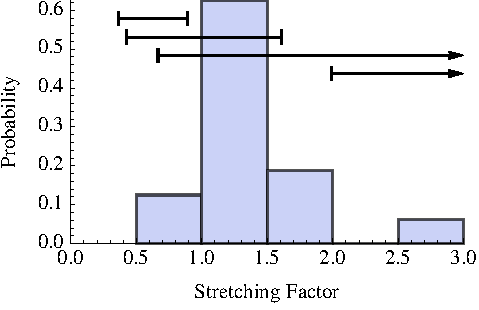
\includegraphics[width=\textwidth]{kappaDistributionHistogram}
		\label{fig:kappaDistributionHistogram}
		\caption{Histogram (blue) obtained from the model. Black error bars show observed stretching factors.}
	\end{subfigure}
	\hfill
	\begin{subfigure}{0.45\textwidth}
		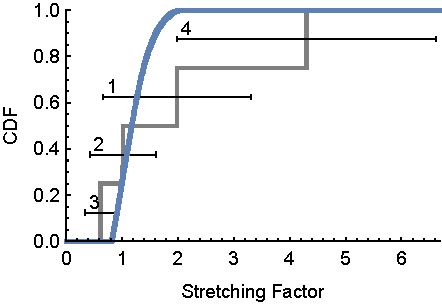
\includegraphics[width=\textwidth]{kappaDistributionCDF}
		\label{fig:kappaDistributionCDF}
		\caption{CDF (blue) obtained from the model. Gray curve and black error bars show observed stretching factors.}
	\end{subfigure}
	\hspace*{\fill}
	\caption{
		Stretching factors histogram and CDF produced by our model.
		The sample contains $4096$ bursts.
		Numbered error bars correspond to GRB 080916C, GRB 090510, GRB 090902B and GRB 090926A (in this order).
	}
	\label{fig:kappaDistribution}
\end{figure}

\begin{figure}
        \centering
        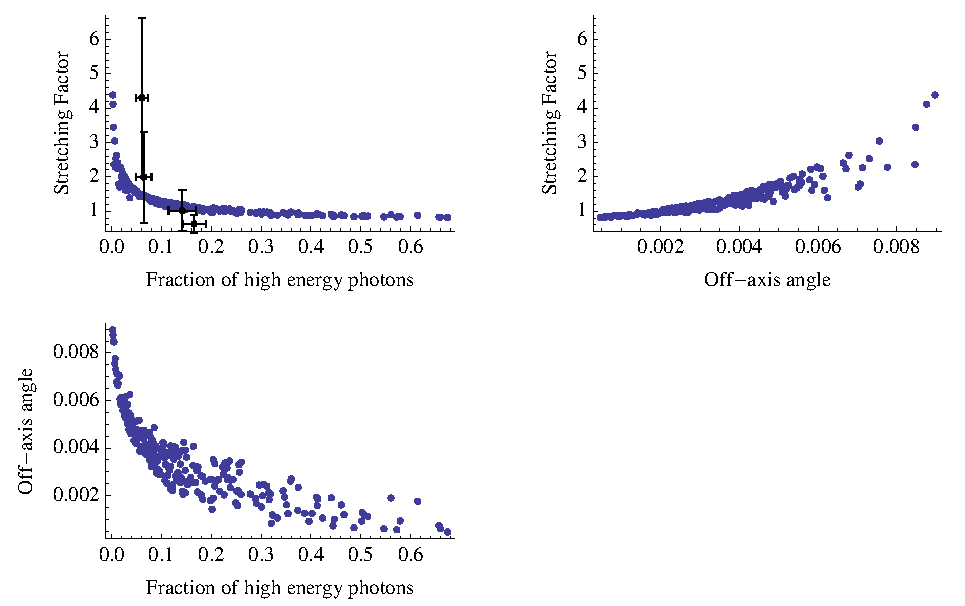
\includegraphics[width=1.0\textwidth]{correlations}
        \caption{
        	Correlations between off-axis angles, stretching factors and high to low energy photon count ratios found in the sample produced by our model.
        	The sample contains $4096$ bursts.
        	Numbered black crosses show data for GRB 080916C, GRB 090510, GRB 090902B and GRB 090926A (in this order) with $2\sigma$ error bars.
        	This correlation allows one to estimate off-axis angles of observed bursts.
        }
        \label{fig:correlations}
\end{figure}

%\section{Conclusions}

%\label{sec:conclusions}
%% TODO: remove section

%% TODO: add more descriptive words

	Our study can be summarized with 3 main conclusions.

	First, the time stretching of GRB light curves between different VHE (in particular $(\unit[100]{MeV}, \unit[1]{GeV})$ and $(\unit[1]{GeV}, \unit[300]{GeV})$) bands is discovered with statistic significance of $3.3\sigma$.
	This time stretching might be positive or negative (that is higher or lower energy light curve is stretched) depending on the burst.

	Second, this time stretching effect can be explained with curvature effects, that is effects of jet geometry.
	There is no need to introduce any new spectral components.

	Finally, we can assume all GRBs to be the same in their rest frames.
	The internal burst parameters (such as $\gamma$, $\eta_0$, $r_0$, $n$, $\omega_0$, $\theta_0$, $k$ and $\alpha$) might stay the same for all bursts, and this assumption is more or less consistent with existing observations.

	However, there are some caveats, and directions for improvement.

	First of all, the model prediction and observations are not completely consistent.
	If you look at fig. \ref{fig:correlations}, you will see that the stretching factor of GRB 090926A is too high compared to the model prediction.
	It appears that parameters of the model cannot be fitted to account for it (without ruining agreement with other observations).
	More data should be analyzed to see whether the problem will be exacerbated, and some refinement of the model might also be required.

	Second, the shapes of light curves produced by the model (see fig. \ref{fig:sampleLightCurves}) differ considerably from observed ones (e.g. fig. \ref{fig:grb090902B}).
	Most importantly, the slope of light curves produced by the model is zero at $t = 0$, even though the slope of observed light curves at $t = 0$ is not only non-zero, but appears to have a maximum.

	Third, the assumption of plasma energy dependence on off-axis angle should be better justified.
	This might probably be done using hydrodynamic simulation of the jet.

	Finally, even though it appears that bursts are similar in their rest frames, they cannot be exactly the same.
	The differences in masses, metallicities, angular momenta of progenitor stars, and the differences in local conditions around them might account for differences in light curves of GRBs (or, even, for especially large stretching factor of GRB 090926A).
	It means that minor variations of model parameters might be necessary on burst per burst basis.

It seems, however, that all these problems are not unresolvable, and
may be addressed by refining the model without changing its main
assumptions.
%% TODO: remove unresolvable, rephrase

{\bf Acknowledgments.} We thank M.~Pshirkov and S.~Troitsky for
comments and inspiring discussions.  The work was supported by Russian
Science Foundation grant 14-12-01340. The analysis is based on data
and software provided by the Fermi Science Support Center (FSSC). The
numerical part of the work was done at the cluster of the Theoretical
Division of INR RAS. G.R. acknowledges the fellowship of the Dynasty
foundation.


\begin{appendices}

\section{Details of using Fermi Science tools}
\label{sec:fermiCode}
This appendix contains two things: exact values we are passing to a web form on the Fermi LAT data server, and the code we use to invoke the Fermi tools (including full list of options).

Parameters that are passed to the web form of the Fermi LAT data server to download the bursts data are the following:
\begin{itemize}
	\item{
		{\bf Object name or coordinates}.
		Coordinates are filled from the table \ref{tab:bursts}.
	}
	\item{
		{\bf Coordinate system}.
		J2000.
	}
	\item{
		{\bf Search radius (degrees)}.
		$60$.
		Events are filtered by location separately by using the point spread functions (PSFs) of the LAT (as described in section \ref{sec:photonSelection}).
	}
	\item{
		{\bf Observation dates}.
		To have a decent safety margin, we extend the duration of the burst by $50\%$ to both past and future relative to the table \ref{tab:bursts} time ranges.
		So, we fill in the following values:
		\begin{align*}
			\texttt{time} + \texttt{startOffset} &- 0.5\left(\texttt{endOffset}-\texttt{startOffset}\right),\\
			\texttt{time} + \texttt{endOffset} &+ 0.5\left(\texttt{endOffset}-\texttt{startOffset}\right)
		\end{align*}
	}
	\item{
		{\bf Time system}.
		MET.
	}
	\item{
		{\bf Energy range (MeV)}.
		$100,\,300000$.
		This includes our both energy ranges.
	}
	\item{
		{\bf LAT data type}.
		Extended.
	}
	\item{
		{\bf Spacecraft data}.
		Checked.
		It is required for both events filtering, and calculation of the PSFs and exposure maps.
	}
\end{itemize}

For background, all parameters are the same, except for the time ranges, which are the following:
\begin{align*}
	\texttt{time} + \texttt{startOffset} &- 0.5\left(\texttt{endOffset} - \texttt{startOffset}\right) - 86400,\\
	\texttt{time} + \texttt{startOffset} &- 0.5\left(\texttt{endOffset} - \texttt{startOffset}\right)
\end{align*}

The commands we use to invoke Fermi Science tools are the following:
\begin{lstlisting}
gtselect infile=[eventFile] outfile=filtered.fits
	ra=INDEF dec=INDEF rad=180 tmin=INDEF tmax=INDEF emin=100 emax=300000
	zmax=100 evclass=2 convtype=-1 evtable=EVENTS
\end{lstlisting}
Here \texttt{[eventFile]} is the file downloaded from the Fermi LAT data server.

\begin{lstlisting}
gtmktime scfile=[spacecraft] sctable=SC_DATA
	filter="DATA_QUAL>0 && LAT_CONFIG==1" roicut=yes
	evfile=filtered.fits evtable=EVENTS outfile=timed.fits
	apply_fiter=yes
\end{lstlisting}
where \texttt{[spacecraft]} is the FITS file containing the spacecraft data (also downloaded from the Fermi LAT data server).

\begin{lstlisting}
gtltcube evfile=timed.fits evtable=EVENTS scfile=[spacecraft] sctable=SC_DATA
	outfile=ltcube.fits
	dcostheta=0.025 binsz=1 phibins=0 tmin=0 tmax=0 zmax=100 zmin=0
\end{lstlisting}

\begin{lstlisting}
gtpsf expcube=ltcube.fits outfile=psf_[IrfName].fits outtable=PSF irfs=[IrfName]
	ra=[RA] dec=[DEC] emin=100 emax=300000 nenergies=41 thetamax=30 ntheta=300
\end{lstlisting}
\texttt{[RA]} and \texttt{[DEC]} here are the coordinates of the burst, and \texttt{[IrfName]} is the Instrument Response Function, which depends on photon's event class (transient, source, clean, or ultraclean) and conversion type (back or front). The list of IRF names can be obtained with the \texttt{gtirfs} tool. We need to compute PSFs for all of them.

\begin{lstlisting}
gtexpcube2 infile=ltcube.fits cmap=none outfile=expcube_[IrfName].fits irfs=[IrfName]
	nxpix=360 nypix=180 binsz=1 coordsys=CEL xref=0 yref=0 axisrot=0
	proj=CAR ebinalg=log emin=100 emax=300000 enumbins=40
	ebinfile=NONE bincalc=EDGE ignorephi=no thmax=180 thmin=0 table=Exposure
\end{lstlisting}
Note, that R.A. coordinates in the \texttt{expcube} FITS files are indexed in reverse order and starting from 180. For example, $\texttt{ra[0]}=180$, $\texttt{ra[1]}=179$, and so on.

\section{Cosmology}
%% TODO: change title
\label{sec:cosmology}
This appendix contains a few formulas we need from cosmology, in particular the area of a photon sphere $A_\text{ph}\left(z\right)$, a sphere over which photons emitted in a particular burst at redshift $z$ are spread; and the volume of the infinitesimal shell surrounding a burst sphere $\dif V\left(z\right)$, a sphere over which bursts at redshift $z$ are distributed.

First of all, the metric of the expanding Universe:
\begin{equation}
\dif s^2 = -\dif t^2 + a^2\left(t\right) \dif r^2 + a^2\left(t\right) r^2 \dif \Omega_2
\end{equation}
We define $a\left(t_\text{obs}\right) = 1$, where $t_\text{obs}$ is the observation time.

We need to understand how the scale factor changes with time. For that we assume that the energy content of the Universe consists of matter $\Omega_m$ and vacuum energy $\Omega_\Lambda$ only, so that the Friedmann equation takes the following form:
\begin{align*}
\left( \frac{\dot{a}\left(t\right)}{a\left(t\right)} \right)^2 &= \Omega_m H_\text{obs}^2 \frac{1}{a^3\left(t\right)} + H_\text{obs}^2 \Omega_\Lambda \\
\dot{a}\left(t\right) &= a\left(t\right) H_\text{obs} \sqrt{\Omega_m\frac{1}{a^3\left(t\right)} + \Omega_\Lambda} \\
\dif t &= \frac{\dif a}{a\left(t\right) H_\text{obs} \sqrt{\Omega_m\frac{1}{a^3\left(t\right)} + \Omega_\Lambda}}
\end{align*}
Here $H_\text{obs} = H\left(t_\text{obs}\right) = \frac{\dot{a}\left( t_\text{obs} \right)}{a\left( t_\text{obs} \right)} = \dot{a}\left( t_\text{obs} \right)$ is the Hubble parameter at the observation time.

We also need to know the areas of two spheres: the photon sphere, a
sphere over which photons emitted in a particular burst are spread;
and the bursts sphere, a sphere over which bursts at a particular
redshift are distributed. These two spheres have the same radii -- a
distance from the observer to the burst, but different centers: the
photon sphere is centered on the burst, while the bursts sphere is
centered on the observer. Also, they have different areas, because the
scale factor differs at locations of burst and observer.
%% TODO rephrase, mention back in time

Let us begin with the photon sphere. This sphere has the origin at $r = 0$ and $t = 0$, at the central engine of a particular burst. Taking $\dif s = 0$ and $\dif \Omega_2 = 0$ in the equation for metric, we get:
\begin{equation*}
\dif r = \frac{\dif t}{a\left(t\right)}
\end{equation*}
And now we integrate over time to find the observer's position:
\begin{align*}
r\left(t_\text{obs}\right) &= \int_0^{t_\text{obs}}\frac{\dif t}{a\left(t\right)} \\
&= \int_{a\left(0\right)}^1\frac{\dif a}{a^2\left(t\right) H_\text{obs} \sqrt{\Omega_m\frac{1}{a^3\left(t\right)} + \Omega_\Lambda}} \\
&= \frac{\, _2F_1\left(\frac{1}{3},\frac{1}{2};\frac{4}{3};-\frac{\Omega_m}{a^3\left(0\right) \Omega_\Lambda }\right)-a\left(0\right) \, _2F_1\left(\frac{1}{3},\frac{1}{2};\frac{4}{3};-\frac{\Omega_m}{\Omega_\Lambda }\right)}{a\left(0\right) H_\text{obs} \sqrt{\Omega_\Lambda }}
\end{align*}
Here $_2F_1\left(a, b; c; z\right) = \frac{\Gamma\left(c\right)}{\Gamma\left(b\right)\Gamma\left(c-b\right)}\int_0^1 \frac{t^{b-1}\left(1-t\right)^{c-b-1}}{\left(1-t z\right)^a} \dif t$ is a hypergeometric function. We can substitute $a\left(0\right) = \frac{1}{1+z}$, so, finally,
\begin{equation}
r\left(z\right) = \frac{\left(1+z\right)\, _2F_1\left(\frac{1}{3},\frac{1}{2};\frac{4}{3};-\frac{\Omega_m}{\Omega_\Lambda}\left(1+z\right)^3\right) - \, _2F_1\left(\frac{1}{3},\frac{1}{2};\frac{4}{3};-\frac{\Omega_m}{\Omega_\Lambda }\right)}{H_\text{obs} \sqrt{\Omega_\Lambda }}
\end{equation}
The area of the photon sphere is then:
\begin{equation}
A_\text{ph}\left(z\right) = 4 \pi a^2\left(t_\text{obs}\right) r^2\left(z\right) = 4 \pi r^2\left(z\right)
\end{equation}

The second sphere is the bursts sphere. It has its origin at the
observer's position, and the radius the same as the photon
sphere. Therefore, its area is:
%% TODO: mention that this is the sphere in the past
\begin{equation}
A_\text{b}\left(z\right) = 4 \pi a^2\left(0\right) r^2\left(z\right) = \frac{4 \pi r^2\left(z\right)}{\left(1+z\right)^2}
\end{equation}

We need to know one more thing about the bursts sphere -- the volume of the infinitesimal shell surrounding it. For that we can again use the metric:
\begin{align}
\dif V\left(z\right) &= - A_\text{b}\left(z\right) a\left(0\right) \dif r \nonumber\\
&= - A_\text{b}\left(z\right) a\left(0\right) \frac{\dif a}{a^2\left(0\right) H_\text{obs} \sqrt{\Omega_m\frac{1}{a^3\left(t\right)} + \Omega_\Lambda}} \nonumber\\
&= A_\text{b}\left(z\right) \frac{\frac{1}{\left(1+z\right)^2}\dif z \left(1+z\right)}{H_\text{obs} \sqrt{\Omega_m\frac{1}{a^3\left(t\right)} + \Omega_\Lambda}} \nonumber\\
&= A_\text{b}\left(z\right) \frac{1}{\left(1+z\right)} \frac{\dif z}{H_\text{obs} \sqrt{\Omega_m\left(1+z\right)^3 + \Omega_\Lambda}} \nonumber\\
&= \frac{4\pi r^2\left(z\right)}{\left(1+z\right)^3} \frac{\dif z}{H_\text{obs} \sqrt{\Omega_m\left(1+z\right)^3 + \Omega_\Lambda}}
\end{align}

\end{appendices}

\bibliographystyle{ieeetr}
\bibliography{gammaRays.bib}

\end{document}
